%%%%%%%%%%%%%%%%%%%%%%%%%%%%%%%%%%%%%%%%%%%%%%%%%%%%%%%%%%%
% --------------------------------------------------------
% Tau
% LaTeX Template
% Version 2.4.4 (28/02/2025)
%
% Author: 
% Guillermo Jimenez (memo.notess1@gmail.com)
% 
% License:
% Creative Commons CC BY 4.0
% --------------------------------------------------------
%%%%%%%%%%%%%%%%%%%%%%%%%%%%%%%%%%%%%%%%%%%%%%%%%%%%%%%%%%%

\documentclass[10pt,a4paper,twocolumn,twoside]{tau-class/tau}
\usepackage[english]{babel}

%% Spanish babel recomendation
% \usepackage[spanish,es-nodecimaldot,es-noindentfirst]{babel} 

%% Draft watermark
% \usepackage{draftwatermark}

%----------------------------------------------------------
% TITLE
%----------------------------------------------------------

\journalname{ELL201 Sem-2 2024-25 Project Report}
\title{CPLD Maths Game using Verilog}

%----------------------------------------------------------
% AUTHORS, AFFILIATIONS AND PROFESSOR
%----------------------------------------------------------


\author[a]{Arnav Singh}
\author[b]{Lakshya Bhatnagar}
\author[c]{Mahesh Pareek}
\author[d]{Arnav Panjla}

%----------------------------------------------------------

\affil[a]{Arnav Singh, 2023EE10968}
\affil[b]{Lakshya Bhatnagar, 2023AM10945}
\affil[c]{Mahesh Pareek, 2023MT10586}
\affil[d]{Arnav Panjla, 2023EE10978}

\professor{\textbf{Prof. Dhiman Malik} \\ \textbf{TA:} Chithambara J}

%----------------------------------------------------------
% FOOTER INFORMATION
%----------------------------------------------------------

\institution{Indian isntitute of technology, Delhi}
\theday{April 29, 2025}
\course{ELL201 Sem-2 2024-25 Project}

%----------------------------------------------------------
% ABSTRACT AND KEYWORDS
%----------------------------------------------------------
\begin{abstract}    
    This project presents the design and implementation of a memory-based arithmetic game on the MAX3000A CPLD using Verilog HDL. The system operates at a 1Hz clock rate and guides players through phases of random number display, sum calculation, input validation, and feedback through LEDs. A dedicated binary-to-BCD module ensures proper formatting for the 7-segment displays. This project reinforces concepts of sequential logic, finite state machines, and modular Verilog design in a real-world CPLD application.
\end{abstract}

%----------------------------------------------------------

\keywords{CPLD, Verilog, Memory Game, Arithmetic Game, LFSR, BCD Conversion}

%----------------------------------------------------------

\begin{document}
		
    \maketitle 
    \thispagestyle{firststyle} 
    \tauabstract 
    % \tableofcontents
    % \linenumbers 
    
%----------------------------------------------------------

\section{Introduction}

    \taustart{T}his project implements a memory-based arithmetic game on the MAX3000A CPLD using Verilog HDL. The system operates on a 1Hz clock, with each game cycle divided into five distinct phases:
    
    \begin{enumerate}
        \item A 5-bit Linear Feedback Shift Register (LFSR) generates pseudo-random numbers, which are displayed one at a time and internally summed.
        \item After displaying the numbers, the screen is cleared to allow the player to input their calculated sum using the onboard switches.
        \item The system then displays the correct sum and compares it to the player's input.
        \item LED indicators provide immediate feedback, showing success or failure through predefined light patterns.
        \item Finally, the system resets automatically to begin a new game round.
    \end{enumerate}

A separate \texttt{binary\_to\_bcd} module handles binary to BCD conversion, enabling correct representation on 7-segment displays.
	
\section{Motivation}

    The goal of this project is to practically apply concepts of Verilog programming, sequential digital design, and modular circuit development on CPLDs. By integrating a memory challenge with arithmetic operations, the project not only reinforces theoretical knowledge but also develops skills related to finite state machines, random number generation using LFSRs, and binary-BCD conversions essential for digital display systems.
    
\section{Implementation Methodology}

    \subsection{Pin Mapping}
    
    The following table summarizes the pin configuration used for interfacing the CPLD with switches, LEDs, 7-segment display outputs, and the clock:

    \begin{figure}[h!]
        \centering
        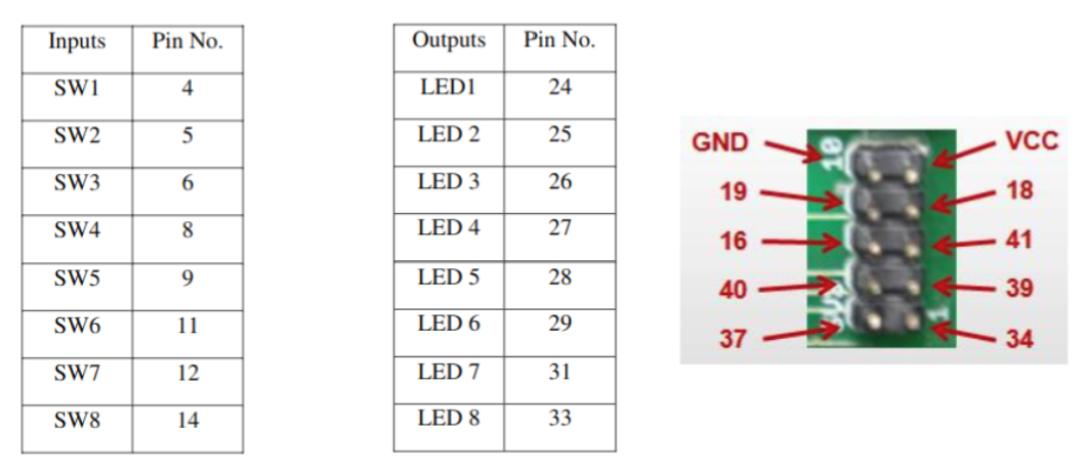
\includegraphics[width=0.52\textwidth]{figures/cpld_pinout.png}
        \caption{MAX3000A pinout for reference}
        \label{fig:circuitdiagram}
    \end{figure}

    \begin{table}[h!]
        \centering
        \begin{tabular}{|c|c|l|}
            \hline
            \textbf{Signal} & \textbf{Pin} & \textbf{Description} \\
            \hline
            clk & 43 & Global clock input (1Hz) \\
            o\_clk & 24 & Debugging clock output \\
            \hline
            bcd\_tens[3] & 34 & BCD tens place output (MSB) \\
            bcd\_tens[2] & 39 & BCD tens place output \\
            bcd\_tens[1] & 41 & BCD tens place output \\
            bcd\_tens[0] & 18 & BCD tens place output (LSB) \\
            bcd\_units[3] & 37 & BCD units place output (MSB) \\
            bcd\_units[2] & 40 & BCD units place output \\
            bcd\_units[1] & 16 & BCD units place output \\
            bcd\_units[0] & 19 & BCD units place output (LSB) \\
            \hline
            switch[7] (rst) & 14 & Reset signal input \\
            switch[6] & 12 & Switch input (bit 6) \\
            switch[5] & 11 & Switch input (bit 5) \\
            switch[4] & 9  & Switch input (bit 4) \\
            switch[3] & 8  & Switch input (bit 3) \\
            switch[2] & 6  & Switch input (bit 2) \\
            switch[1] & 5  & Switch input (bit 1) \\
            switch[0] & 4  & Switch input (bit 0) \\
            \hline
            led[6] & 33 & LED indicator (MSB) \\
            led[5] & 31 & LED indicator \\
            led[4] & 29 & LED indicator \\
            led[3] & 28 & LED indicator \\
            led[2] & 27 & LED indicator \\
            led[1] & 26 & LED indicator \\
            led[0] & 25 & LED indicator (LSB) \\
            \hline
        \end{tabular}
        \caption{Pin Mapping of MAX3000A as done in software}
        \label{tab:pinmapping}
    \end{table}
    
    \subsection{Truth Table and Circuit Diagram}
    
    The truth table and Circuit Diagram below outlines the system behavior during various phases of the game based on the cycle counter value:
    \vspace{15pt}
    \\
    Note - all the data are taken when seed phrase is 10101, for other seed the value will be different.

    \begin{table*}[tp]
        \centering
        \begin{tabular}{|c|c|c|c|}
            \hline
            \textbf{Cycle Counter} & \textbf{Action} & \textbf{Display Output} & \textbf{LED Status} \\
            \hline
            0-3 & Generate random number (LFSR) & Random value & Reflect LFSR value (padded) \\
            4 & Clear display & 0 & OFF \\
            5-10 & Accept user input via switches & Switch value & OFF \\
            11-12 & Display correct answer & Sum modulo 100 & LEDs ON (success or pattern) \\
            13-14 & Hold result display & Sum modulo 100 & LEDs remain in previous state \\
            15 & Reset game & 0 & LEDs ON \\
            \hline
        \end{tabular}
        \caption{Truth Table for Game Phases}
        \label{tab:truthtable}
    \end{table*}
    
    \begin{table*}[!t]
    \centering
        \begin{tabular}{|c|c|c|c|}
            \hline
            \textbf{Step} & \textbf{LFSR State (Binary)} & \textbf{Decimal Equivalent} & \textbf{Feedback (bit4 XOR bit2)} \\
            \hline
            0  & 10101 & 21 & 1 $\oplus$ 1 = 0 \\
            1  & 01010 & 10 & 0 $\oplus$ 0 = 0 \\
            2  & 10100 & 20 & 1 $\oplus$ 1 = 0 \\
            3  & 01000 & 8  & 0 $\oplus$ 0 = 0 \\
            4  & 10000 & 16 & 1 $\oplus$ 0 = 1 \\
            5  & 00001 & 1  & 0 $\oplus$ 0 = 0 \\
            6  & 00010 & 2  & 0 $\oplus$ 0 = 0 \\
            7  & 00100 & 4  & 0 $\oplus$ 1 = 1 \\
            8  & 01001 & 9  & 0 $\oplus$ 0 = 0 \\
            9  & 10010 & 18 & 1 $\oplus$ 0 = 1 \\
            10 & 00101 & 5  & 0 $\oplus$ 1 = 1 \\
            11 & 01011 & 11 & 0 $\oplus$ 0 = 0 \\
            12 & 10110 & 22 & 1 $\oplus$ 1 = 0 \\
            13 & 01100 & 12 & 0 $\oplus$ 1 = 1 \\
            14 & 11001 & 25 & 1 $\oplus$ 0 = 1 \\
            15 & 10011 & 19 & 1 $\oplus$ 0 = 1 \\
            16 & 00111 & 7  & 0 $\oplus$ 1 = 1 \\
            17 & 01111 & 15 & 0 $\oplus$ 1 = 1 \\
            18 & 11111 & 31 & 1 $\oplus$ 1 = 0 \\
            19 & 11110 & 30 & 1 $\oplus$ 1 = 0 \\
            20 & 11100 & 28 & 1 $\oplus$ 1 = 0 \\
            21 & 11000 & 24 & 1 $\oplus$ 0 = 1 \\
            22 & 10001 & 17 & 1 $\oplus$ 0 = 1 \\
            23 & 00011 & 3  & 0 $\oplus$ 0 = 0 \\
            24 & 00110 & 6  & 0 $\oplus$ 1 = 1 \\
            25 & 01101 & 13 & 0 $\oplus$ 1 = 1 \\
            26 & 11011 & 27 & 1 $\oplus$ 0 = 1 \\
            27 & 10111 & 23 & 1 $\oplus$ 1 = 0 \\
            28 & 01110 & 14 & 0 $\oplus$ 1 = 1 \\
            29 & 11101 & 29 & 1 $\oplus$ 1 = 0 \\
            30 & 11011 & 27 & 1 $\oplus$ 0 = 1 \\
            31 & 10111 & 23 & 1 $\oplus$ 1 = 0 \\
            \hline
        \end{tabular}
    \caption{Truth table showing the complete cycle of the 5-bit LFSR starting from 10101 as seed.}
    \end{table*}


    \begin{figure*}[!t]
        \centering
        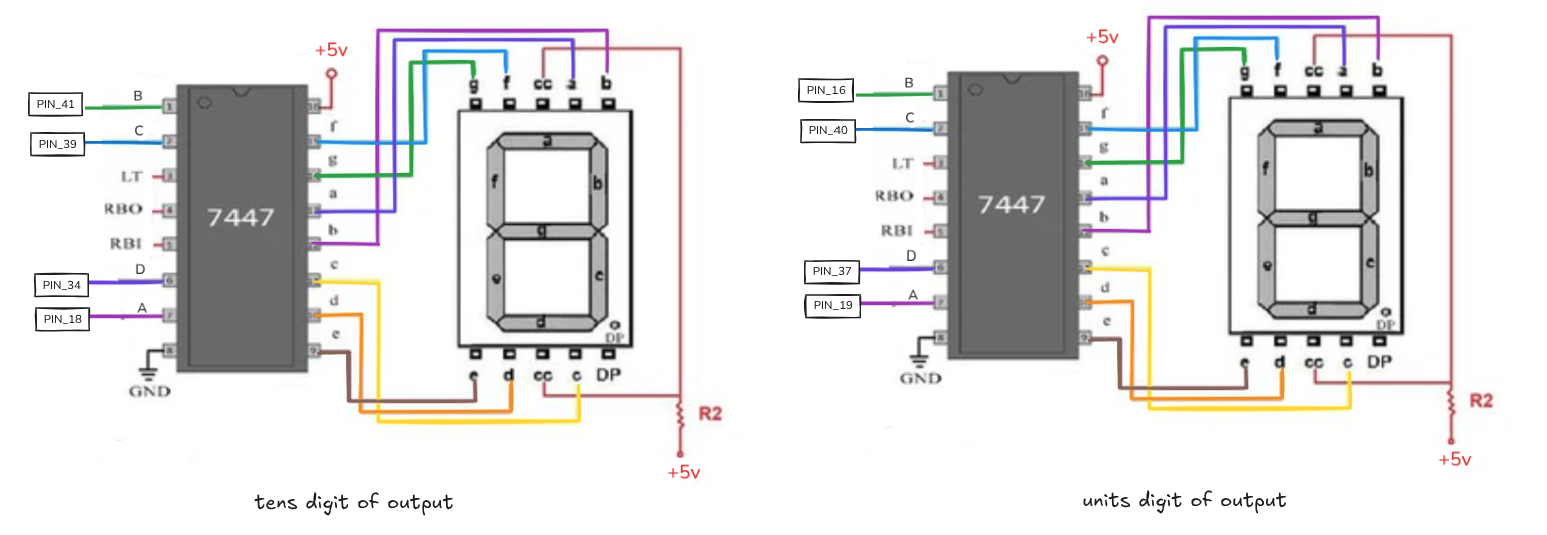
\includegraphics[width=.83\textwidth]{figures/circuit_diagram.png}
        \caption{CPLD Maths Game Circuit Diagram and IO Mapping}
        \label{fig:circuitdiagram}
    \end{figure*}

\section{Test Bench Waveforms}

    \subsection{Tables}
	
        Table \ref{tab:table} shows an example table. The \verb|\tabletext{}| is used to add notes to tables easily. 
    		
        \begin{table}[H]
            \centering
            \caption{Astronomical Object Data}
            \label{tab:table}
            \begin{tabular}{ll}
                \toprule
                \textbf{Object} & \textbf{Distance (Light Years)} \\
                \midrule
                Alpha Centauri & 4.37 \\
                Betelgeuse & 642.5 \\
                Andromeda Galaxy & 2.537 million \\
                \bottomrule   
            \end{tabular}
			
            \tabletext{Note: The table contains data of some famous celestial objects.}
			
        \end{table}

		
\section{Tau packages}

    \subsection{Tauenvs}
	
        This template has its own environment package designed to enhance the presentation of the document. Among these custom environments
		
        There are two environments which have a predefined title. These can be included by the commands
		
    \subsection{Taubabel}

        In previous versions, we included a package called, which have all the commands that automatically translate from English to Spanish when this language package is defined. 
        
        By default, tau displays its content in English. However, at the beginning of the document you will find a recommendation when writing in Spanish. 
		
       You may modify this package if you want to use other language than English or Spanish. This will make easier to translate the document without having to modify the class document.


\newpage

\section{Linear Feedback Shift Register, LFSR Logic }

    In this project, a 5-bit Linear Feedback Shift Register (LFSR) is used to generate pseudo-random numbers for the game. The LFSR advances based on a feedback polynomial that defines which bits are XORed together to create the next input.

    The feedback logic can be described by Equation~\ref{eq:lfsr}:
    
    \begin{equation} \label{eq:lfsr}
        \text{next\_bit} = \text{lfsr}[4] \oplus \text{lfsr}[2]
    \end{equation}

    At every clock cycle, the LFSR shifts its bits to the right by one position, and the newly generated \texttt{next\_bit} is inserted into the most significant bit (MSB) position. This mechanism ensures a repeating but seemingly random sequence of numbers, suitable for a simple memory-based game.
    \\
    The feedback taps (bits 4 and 2) correspond to a primitive polynomial, ensuring maximal sequence length before repetition.

	
\section{Verilog codes}
	
    \lstinputlisting[caption=Example of Matlab code., language=Verilog,label=code]{example.m}
	




%----------------------------------------------------------

\end{document}